\subsection{Data set}

\begin{frame}{NorESM}

    \(1000\) year long simulation run from the \alert{Norwegian Earth System Model
    (NorESM)}

    \begin{figure}
        \centering
        \includegraphics[width=\linewidth]{noresm/noresm_raw_dark.pdf}
        % \only<1>{\inputpgf[.5]{../figures/noresm.pgf}}
        % \only<2>{\inputpgf[.5]{../figures/noresm_zoom.pgf}}
    \end{figure}

    \note<+>{
        \begin{itemize}
            \item The dataset that is used is from the NorESM, with 1000 year long
                simulation of temperature respons to volcanic forcing
            \item Note the difference in the left and right axis, a factor ten difference
            \item The temperature is monthly resolved while the forcing is yearly resolved
        \end{itemize}
    }

\end{frame}

% How forcing is sampled from yearly to monthly
% \newcounter{prep_note_count}
% \begin{frame}{Preparing NorESM data}

%     \begin{figure}
%         \centering
%         % \inputpgf{../figures/noresm_frc_dark.pgf}
%         \includegraphics[width=\linewidth]{../figures/noresm_frc_dark.pdf}
%     \end{figure}

%     \note{
%         Two approaches:
%         \begin{enumerate}
%             \item Expand forcing by repeating elements to monthly resolution (original is the dotted signal)
%                 \setcounter{prep_note_count}{\value{enumi}}
%         \end{enumerate}
%     }

% \end{frame}

% \begin{frame}
%   \frametitle{Historical forcing data}

%   Forcing data from \cite{jones2004} %and \cite{crowley2003}
%   over the last two millennia

%   \begin{figure}
%     \centering
%     % \inputpgf{../figures/jonesmann.pgf}
%     \includegraphics[width=\linewidth]{../figures/jonesmann.pdf}
%   \end{figure}

% \end{frame}

% \begin{frame}
%   \frametitle{Historical temperature data}

%   Temperature data from \cite{2019_pages2k} over the last two millennia

%   \begin{figure}
%     \centering
%     % \inputpgf{../figures/pages2k.pgf}
%     \includegraphics[width=\linewidth]{../figures/pages2k.pdf}
%   \end{figure}

% \end{frame}

\begin{frame}{Proxy data}

    Forcing and temperature data from \cite{jones2004} and \cite{2019_pages2k}
    of the last two millennia

    \begin{figure}
        \centering
        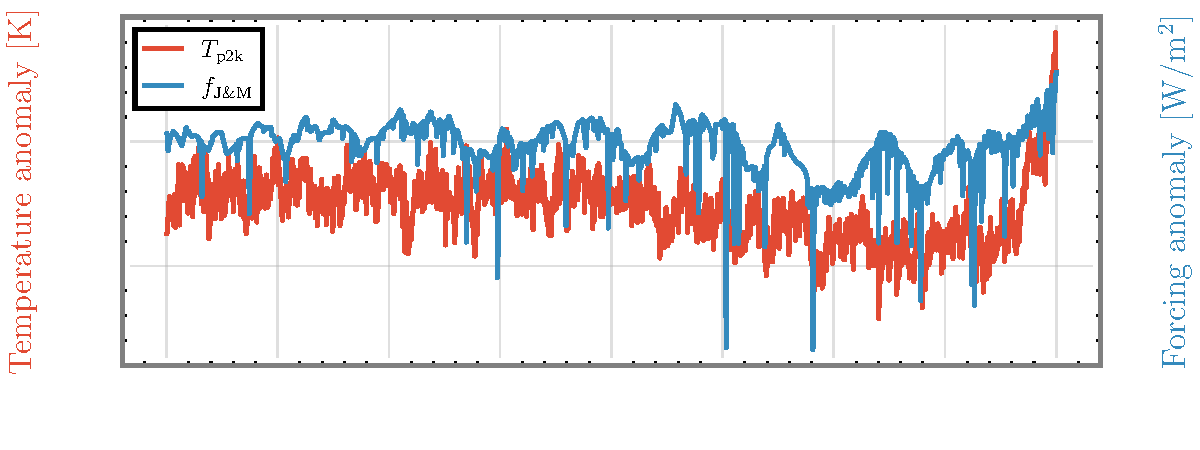
\includegraphics[width=\linewidth]{noresm/raw_historical_beam.pdf}
    \end{figure}

    \note<+>{
        \begin{itemize}
            \item When the response function is obtained, it is tested against
                historical forcing and temperature records inferred from proxy data
            \item Forcing consist of GHG, solar, aerosols, volcanic
            \item Temperature is mean from \(7000\) reconstructions based on proxy data
                from ice cores, tree rings, speleothems, sediments, documentary archives
                and other
        \end{itemize}
    }

\end{frame}
